\documentclass[11pt,oneside]{amsart}
\usepackage{geometry}
\usepackage[T1]{fontenc}
\usepackage{lmodern}
\usepackage{booktabs,pdfpages,parskip}

\pagestyle{empty}

\title{Instructor's Report, Spring 2022\\ \today}

\begin{document}
\maketitle

\bigskip

\textbf{Course number, name:} MATH2211, Honors Linear Algebra

\textbf{Instructor:} Yongyi Chen

\section{Report}
\subsection{Texts}
A combination of Bill Keane's 2019S linear algebra notes and Axler's \emph{Linear Algebra Done Right}. 

\subsection{Topics (include sections of text)}
\begin{itemize}
    \item Introduction, set theory, intro to proofs, proofs by induction
    \item Fields, complex numbers, finite fields
    \item Vector spaces over a field, subspaces, spans
    \item Linear independence, bases, dimension,
    \item Functions, linear transformations, matrices
    \item Kernel, image, rank, nullity
    \item Isomorphisms, change of basis
    \item Solving linear equations
    \item Intro to determinants
    \item Determinants via the exterior algebra
    \item Dual vector spaces, annihilator, the four fundamental subspaces
    \item Eigenvalues, characteristic polynomial, eigenspaces, trace
    \item Inner products, orthonormal bases, Riesz representation theorem
    \item Projections, adjoints, self-adjoint operators
    \item (Not on final exam) Sneak peek of spectral graph theory and Markov chains
\end{itemize}

\subsection{Some comments about the text}
Between Keane's notes and Axler's book, the students had no problems with the text and using it to solve their homework problems. Both resources were precisely and concisely written. The exercises in Keane's notes are on the easy side, but I had no trouble creating harder problems on my own.

Notably missing from both texts is a unified approach to determinants. Keane's notes takes the ad-hoc computational approach, defining determinants by a cofactor expansion algorithm, while Axler avoids the discussion of determinants until eigenvalues are developed. I took the approach of defining determinants via the exterior algebra and wrote up some notes for this. The exterior algebra approach makes the proofs of most properties of determinants self-evident. However, the caveat is that some students found the exterior algebra content somewhat difficult---perhaps the hardest topic of the course.

Also missing from Keane's notes are quotients, duals, and products. Of these three topics I only discussed duals. It would be nice, although possibly too ambitious, to try to cover more than that.

\subsection{Course format}
In-person, one-hour lectures 3 times per week.

\subsection{Number of exams}
Two midterm exams (50 minutes) and one final exam (3 hours). All were done in person, and all were open notes.

\subsection{Enrollment}
10.

\subsection{Grading policy}
\begin{itemize}
    \item 20\% homework,
    \item 20\% first exam,
    \item 20\% second exam,
    \item 40\% final.
\end{itemize}

\subsection{General comments about this course}
The course was a very big success. I was able to cover a strict superset of what has been covered in the past. The new topics included exterior algebra, dual spaces, the four fundamental subspaces, projections, self-adjoint operators, and the spectral theorem. The students overall handled all of these topics just fine.

\subsection{Final grade distribution}
\begin{itemize}
    \item 5 A
    \item 1 A$-$
    \item 1 B$+$
    \item 2 B
    \item 1 C$+$
\end{itemize}

\vskip 0pt plus 1fill minus 0pt
\noindent
\textbf{Attached are the syllabus, all tests (including final), list of
  HW assignments, and any other pertinent material.} 
\newpage

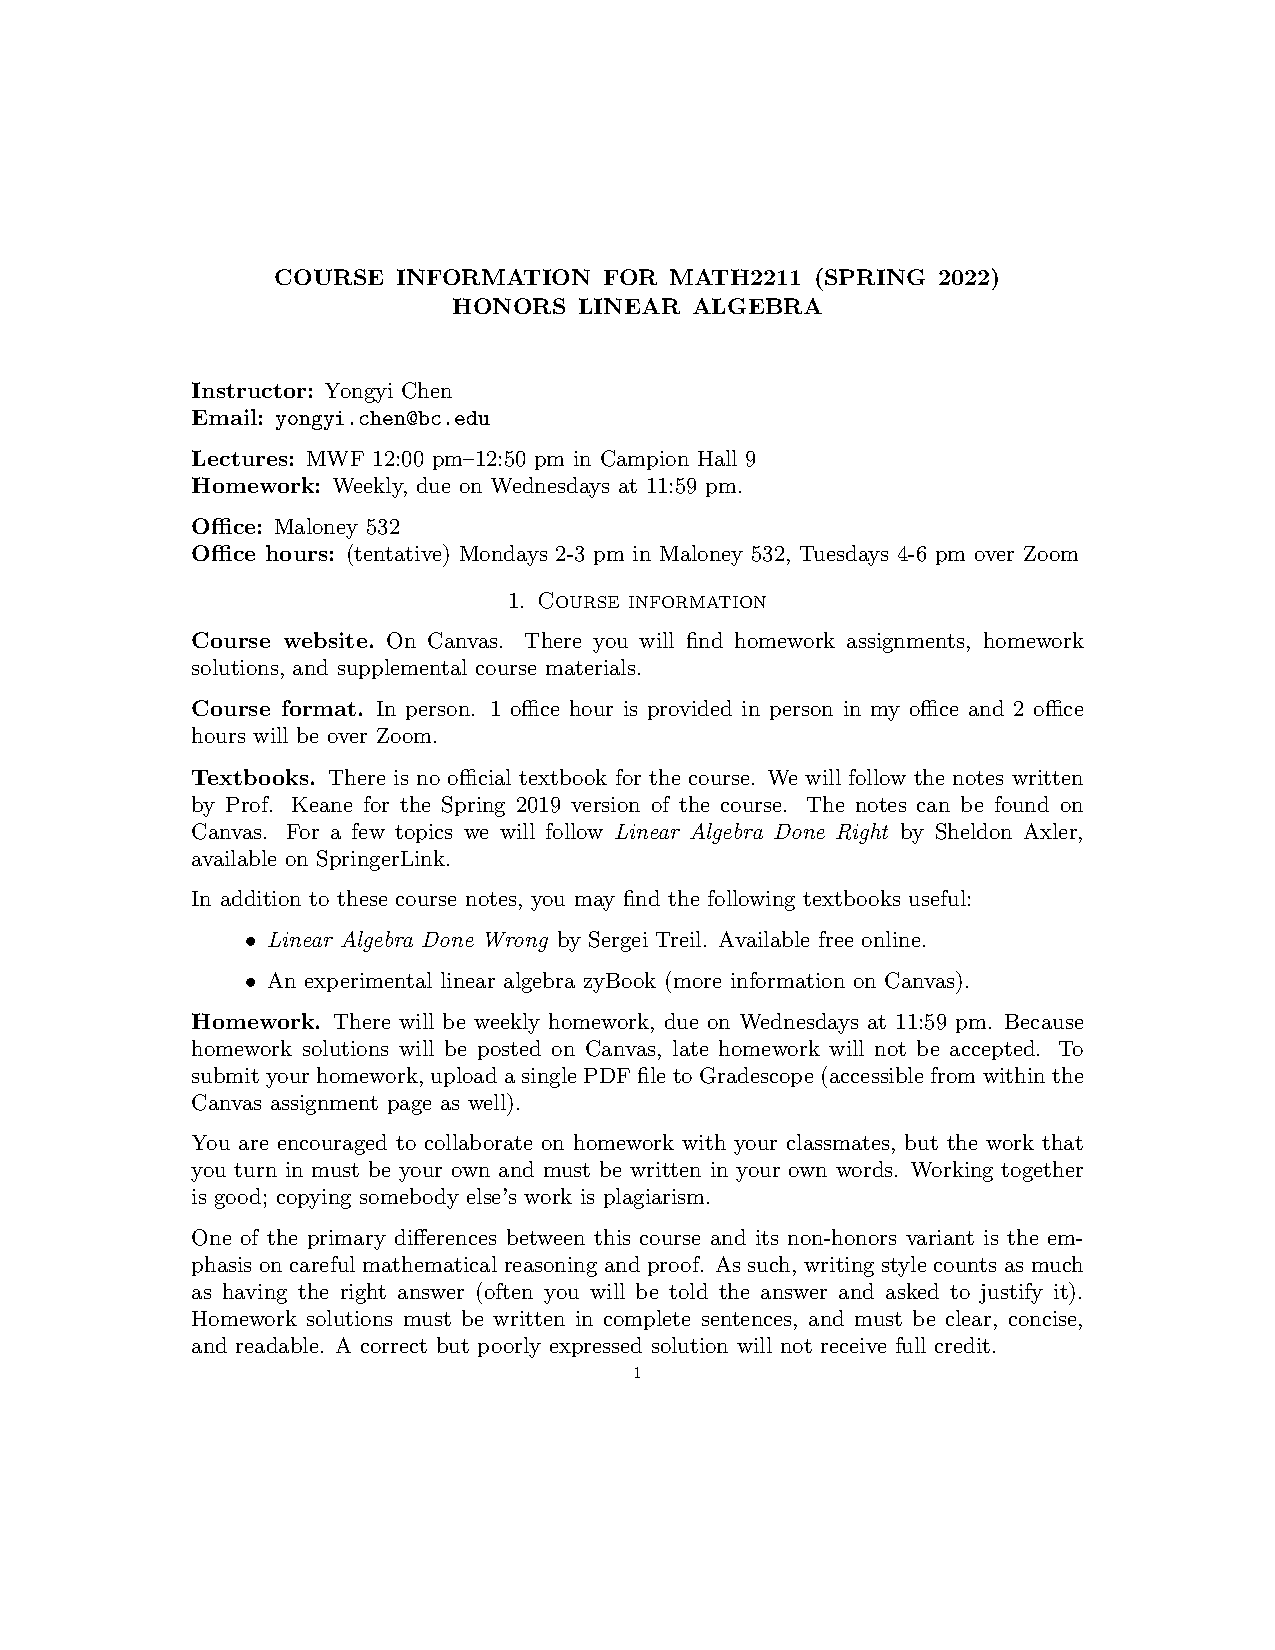
\includepdf[pages=-]{syllabus.pdf}
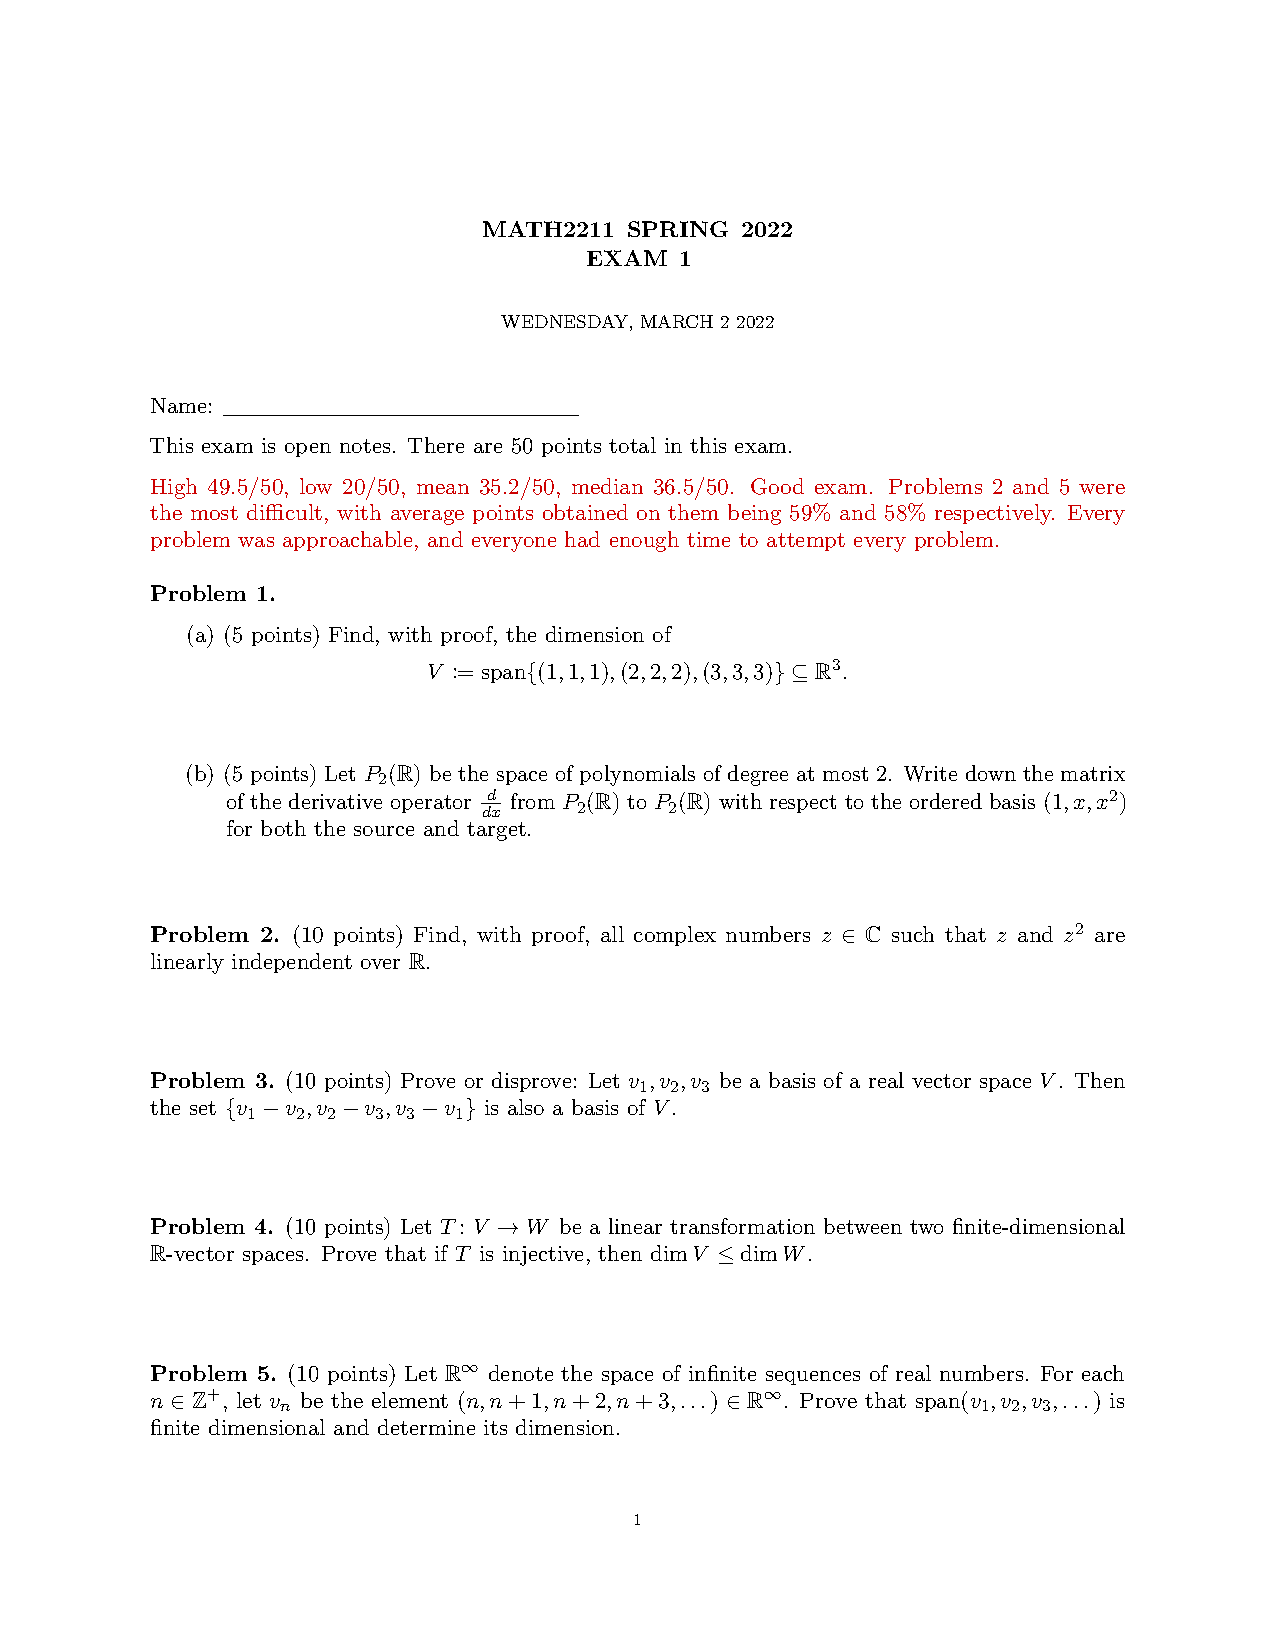
\includepdf[pages=-]{exam1/exam1_annotated.pdf}
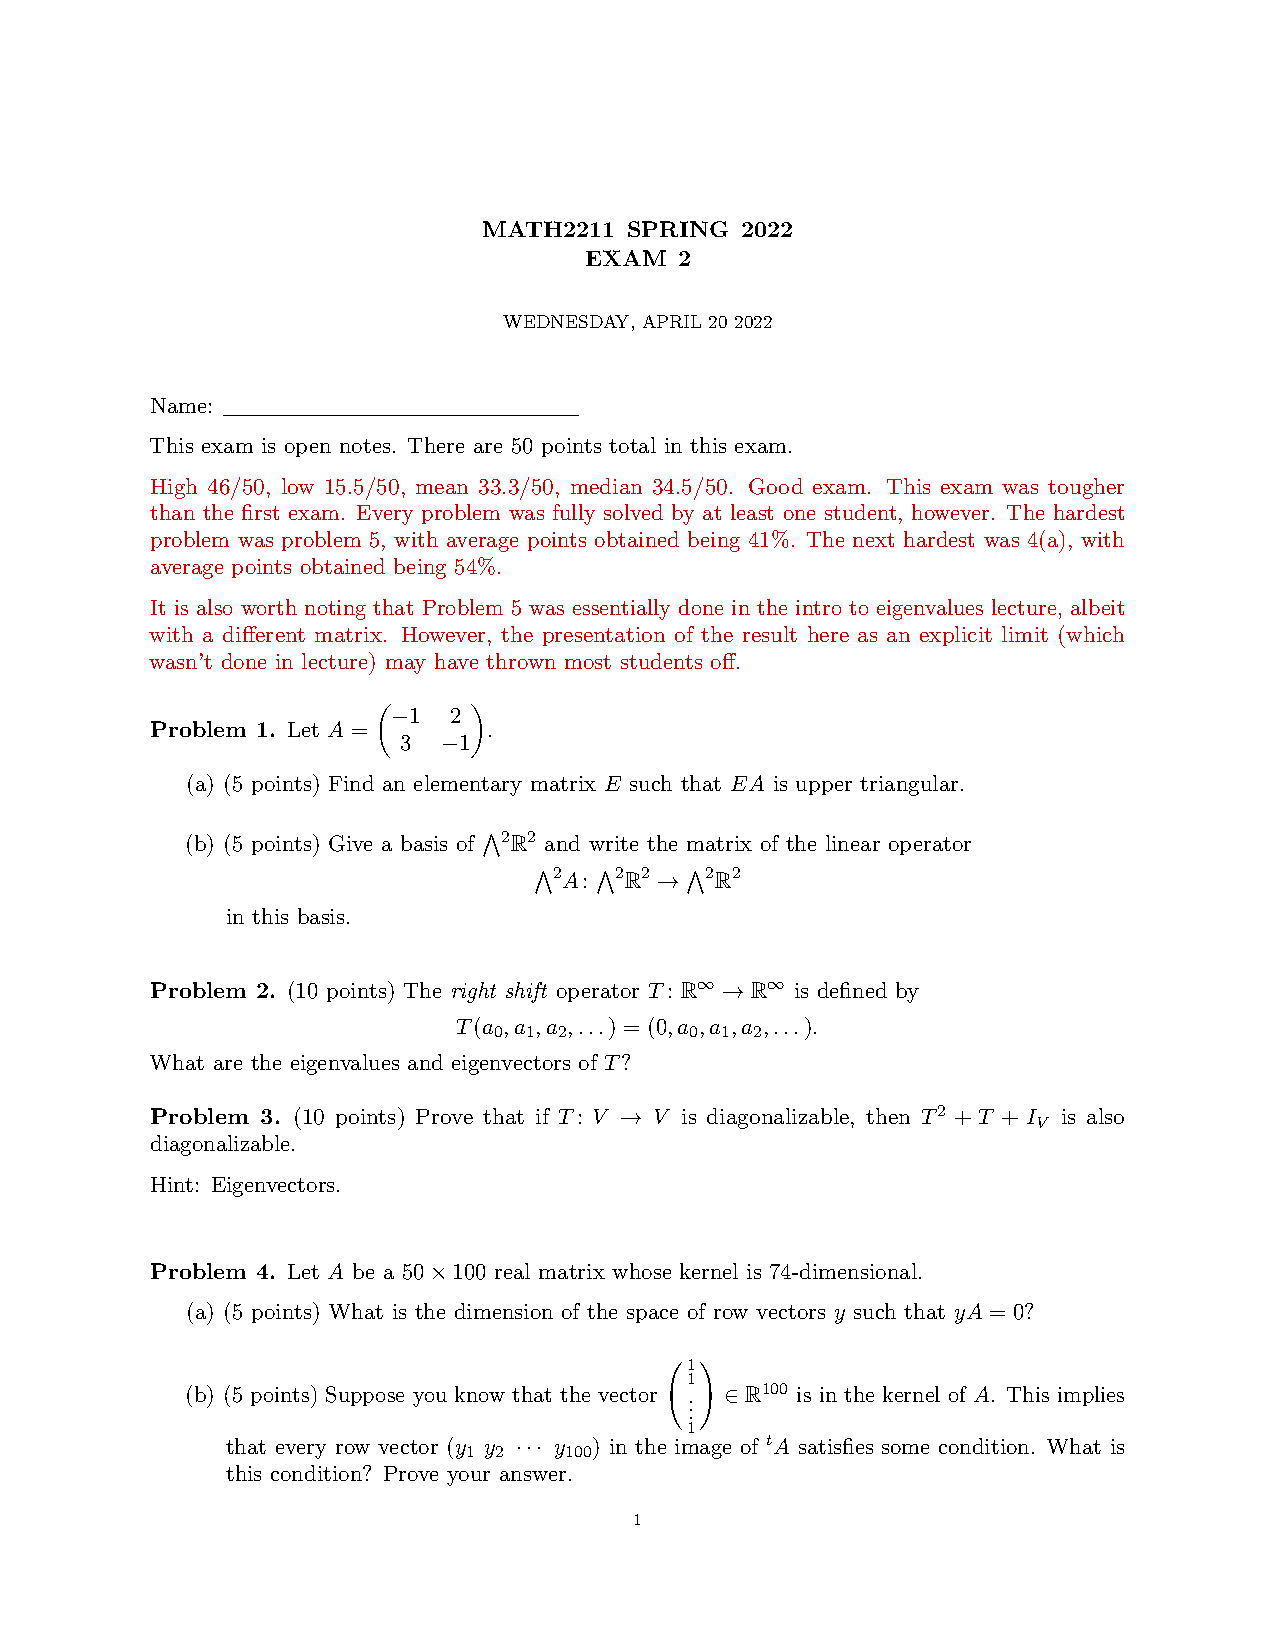
\includepdf[pages=-]{exam2/exam2_annotated.pdf}
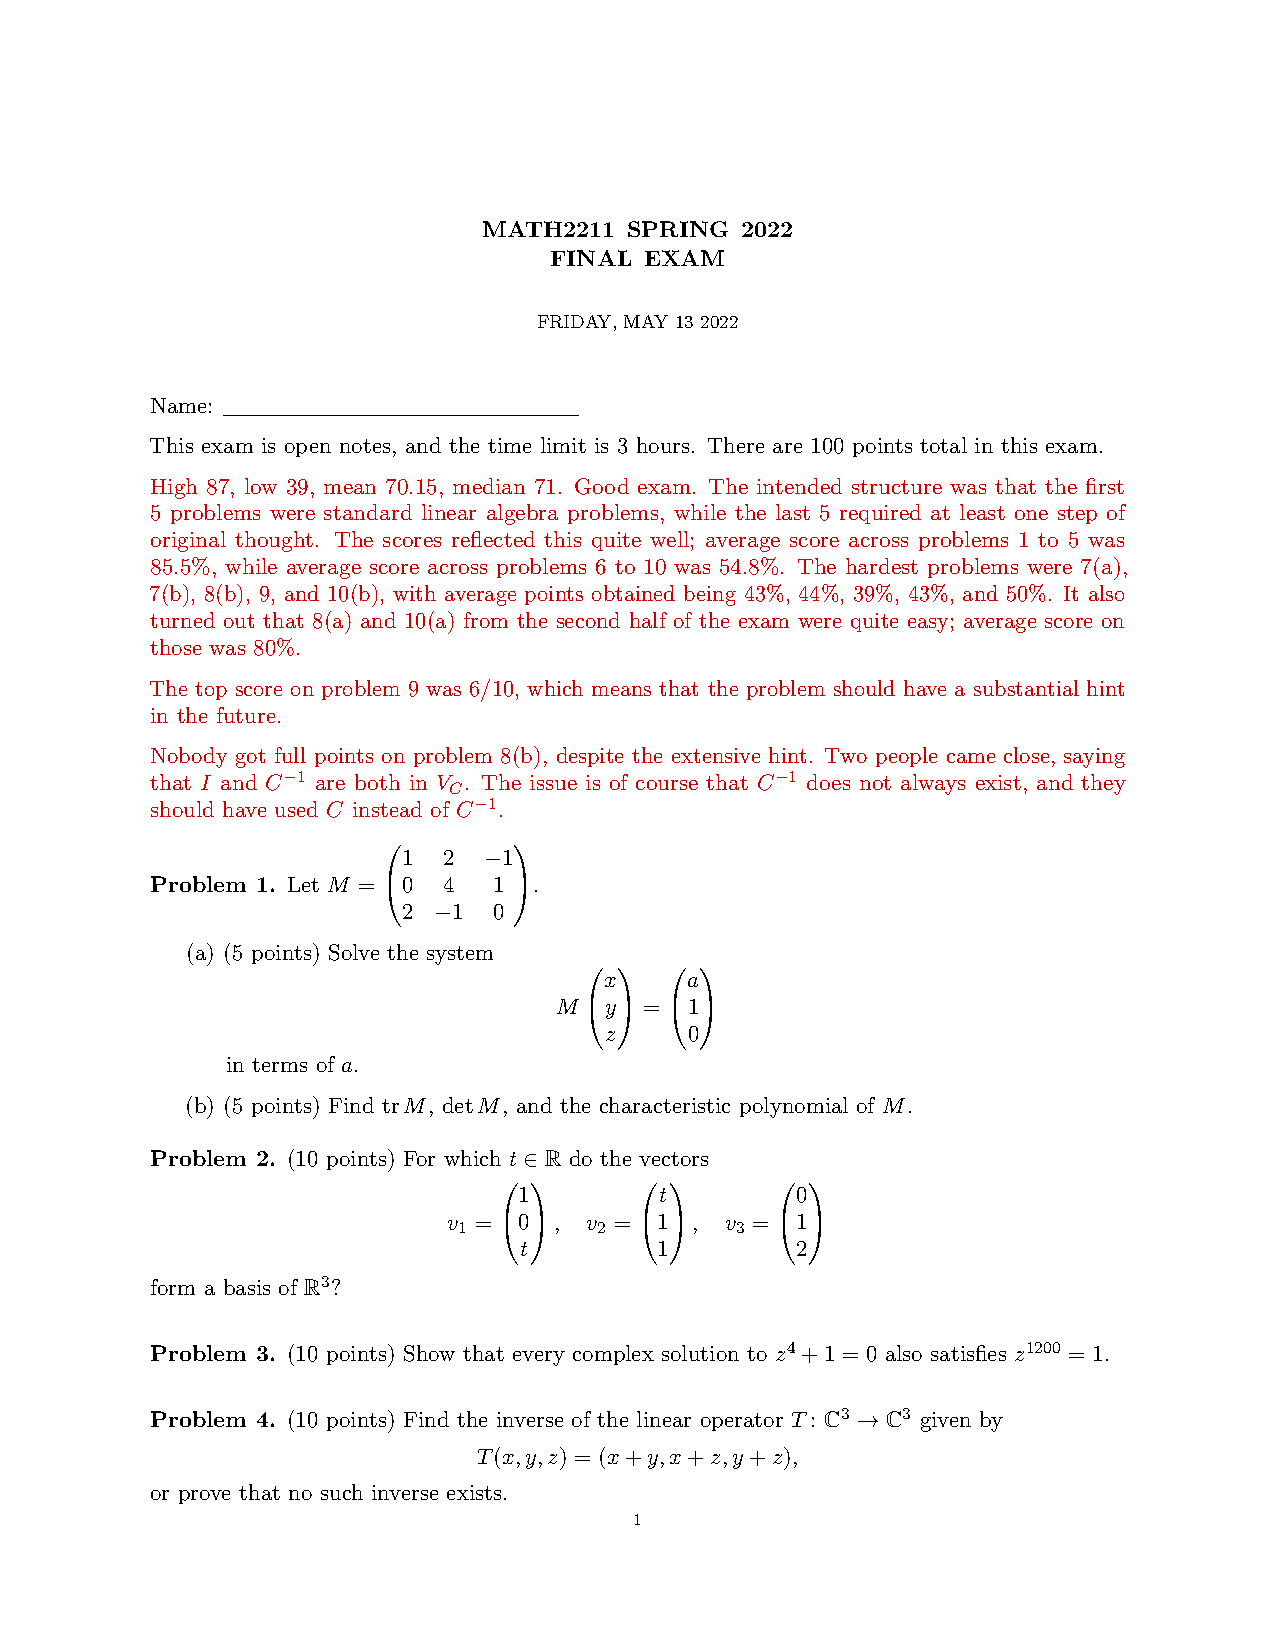
\includepdf[pages=-]{final_exam/final_exam_annotated.pdf}

% Attach psets 1 through 10.
\newcounter{int}
\setcounter{int}{1}
\loop
    \includepdf[pages=-]{pset\theint/pset\theint.pdf}
    \addtocounter{int}{1}
\ifnum \value{int}<11
\repeat

\appendix
\section{Supplementary materials}
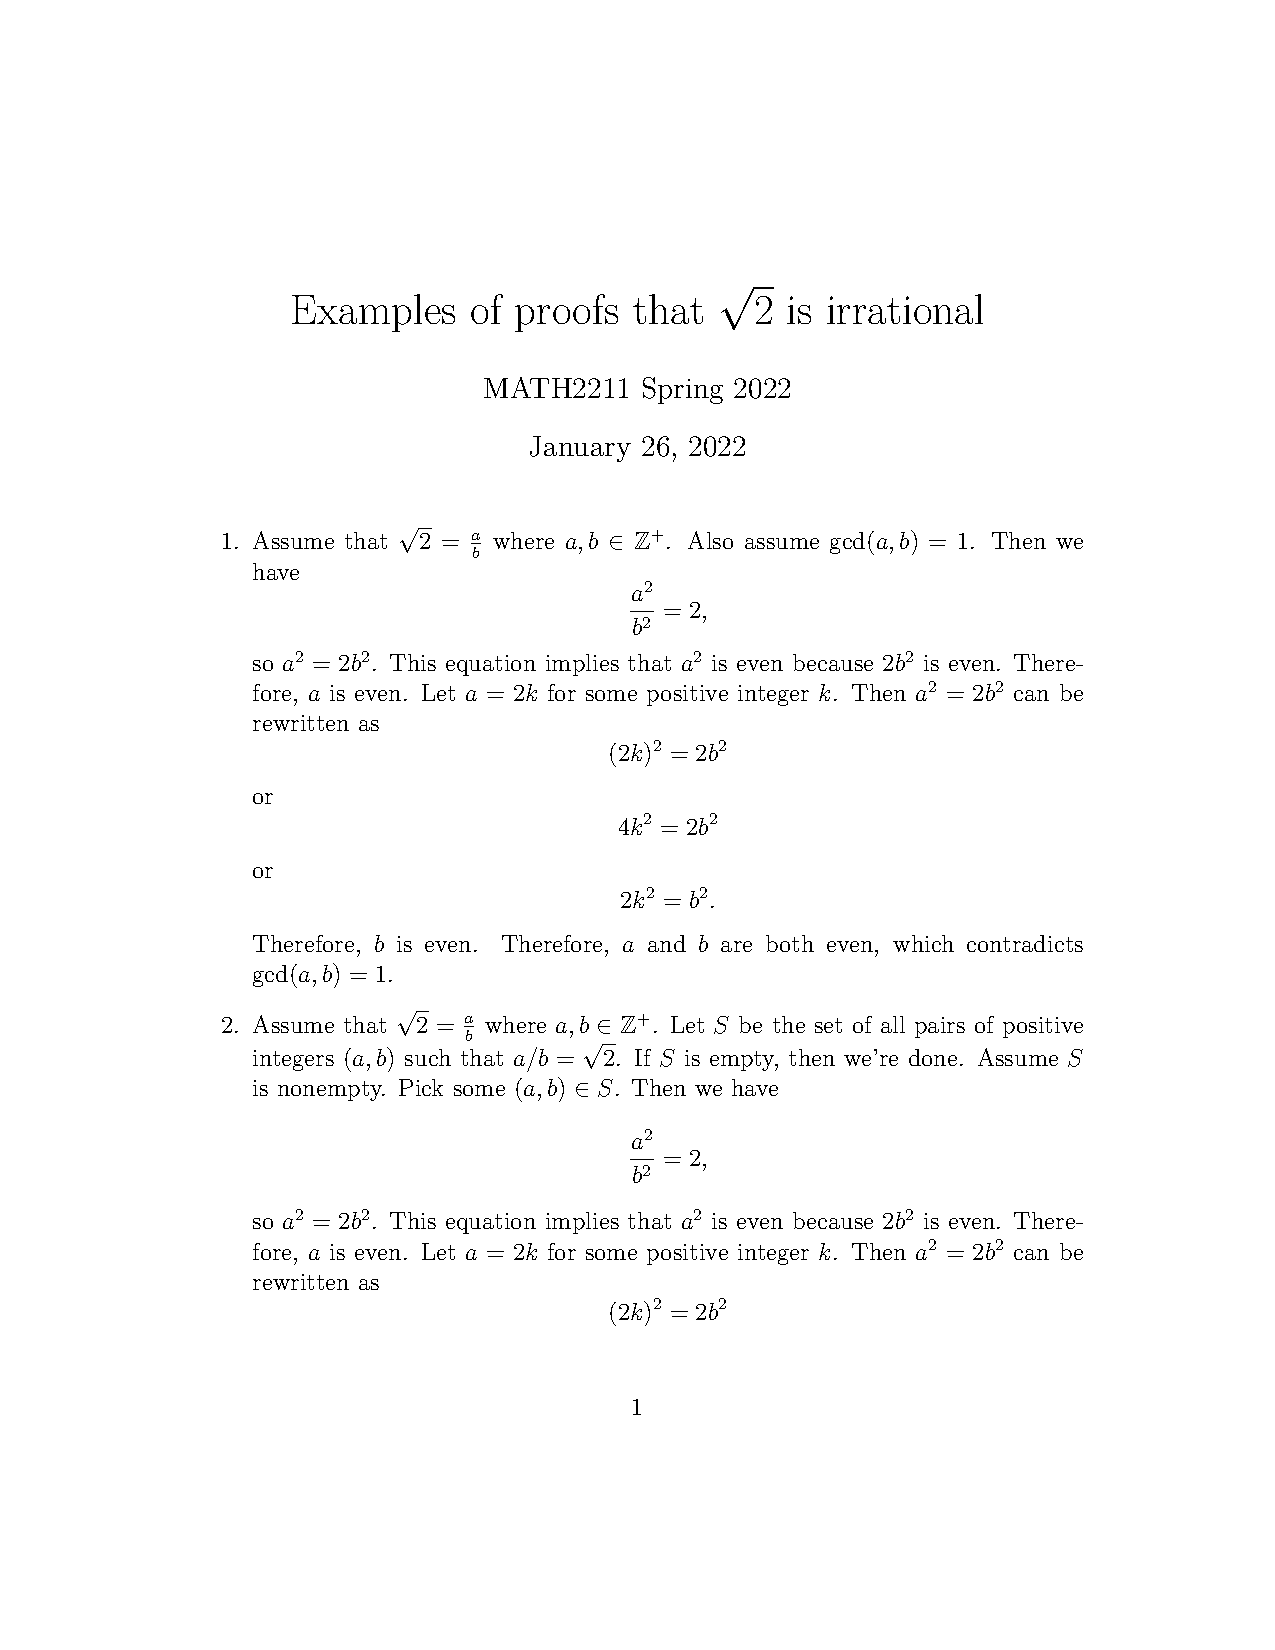
\includepdf[pages=-]{sqrt2.pdf}
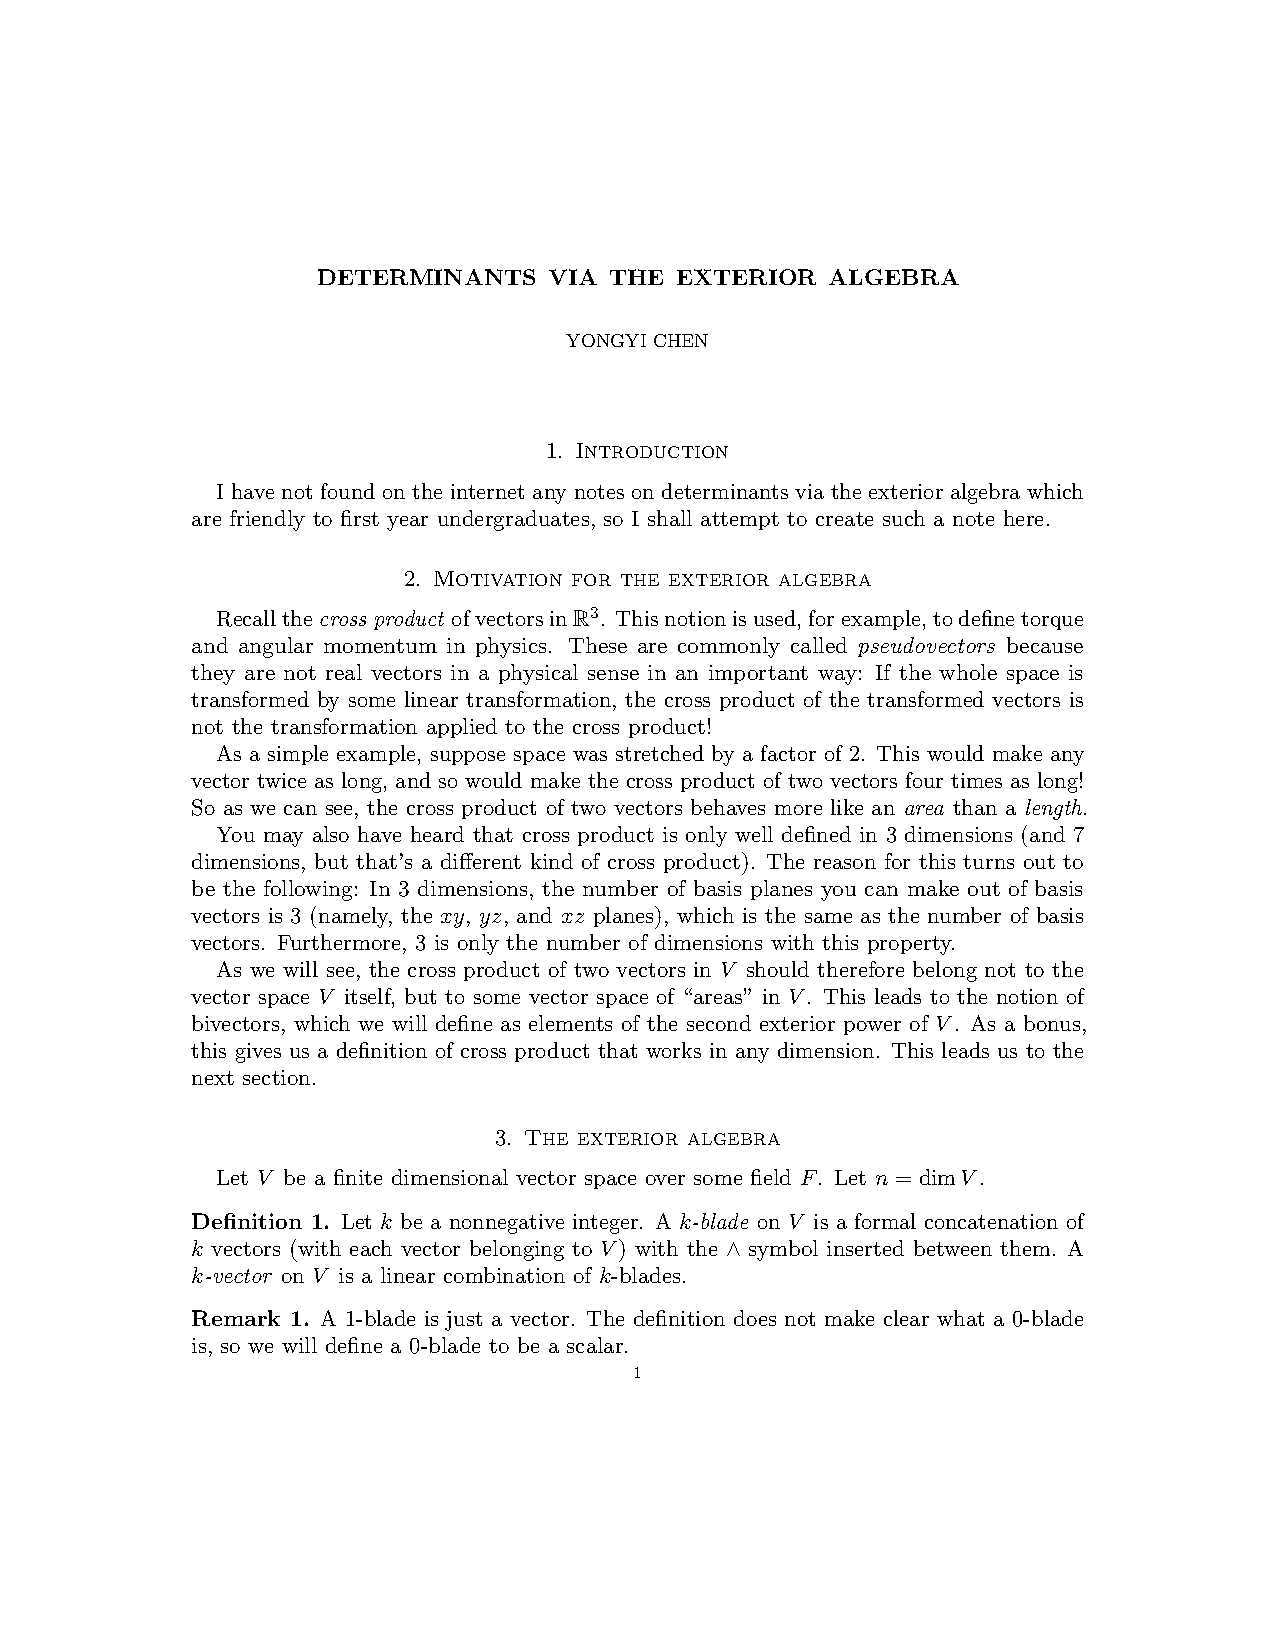
\includepdf[pages=-]{determinant.pdf}
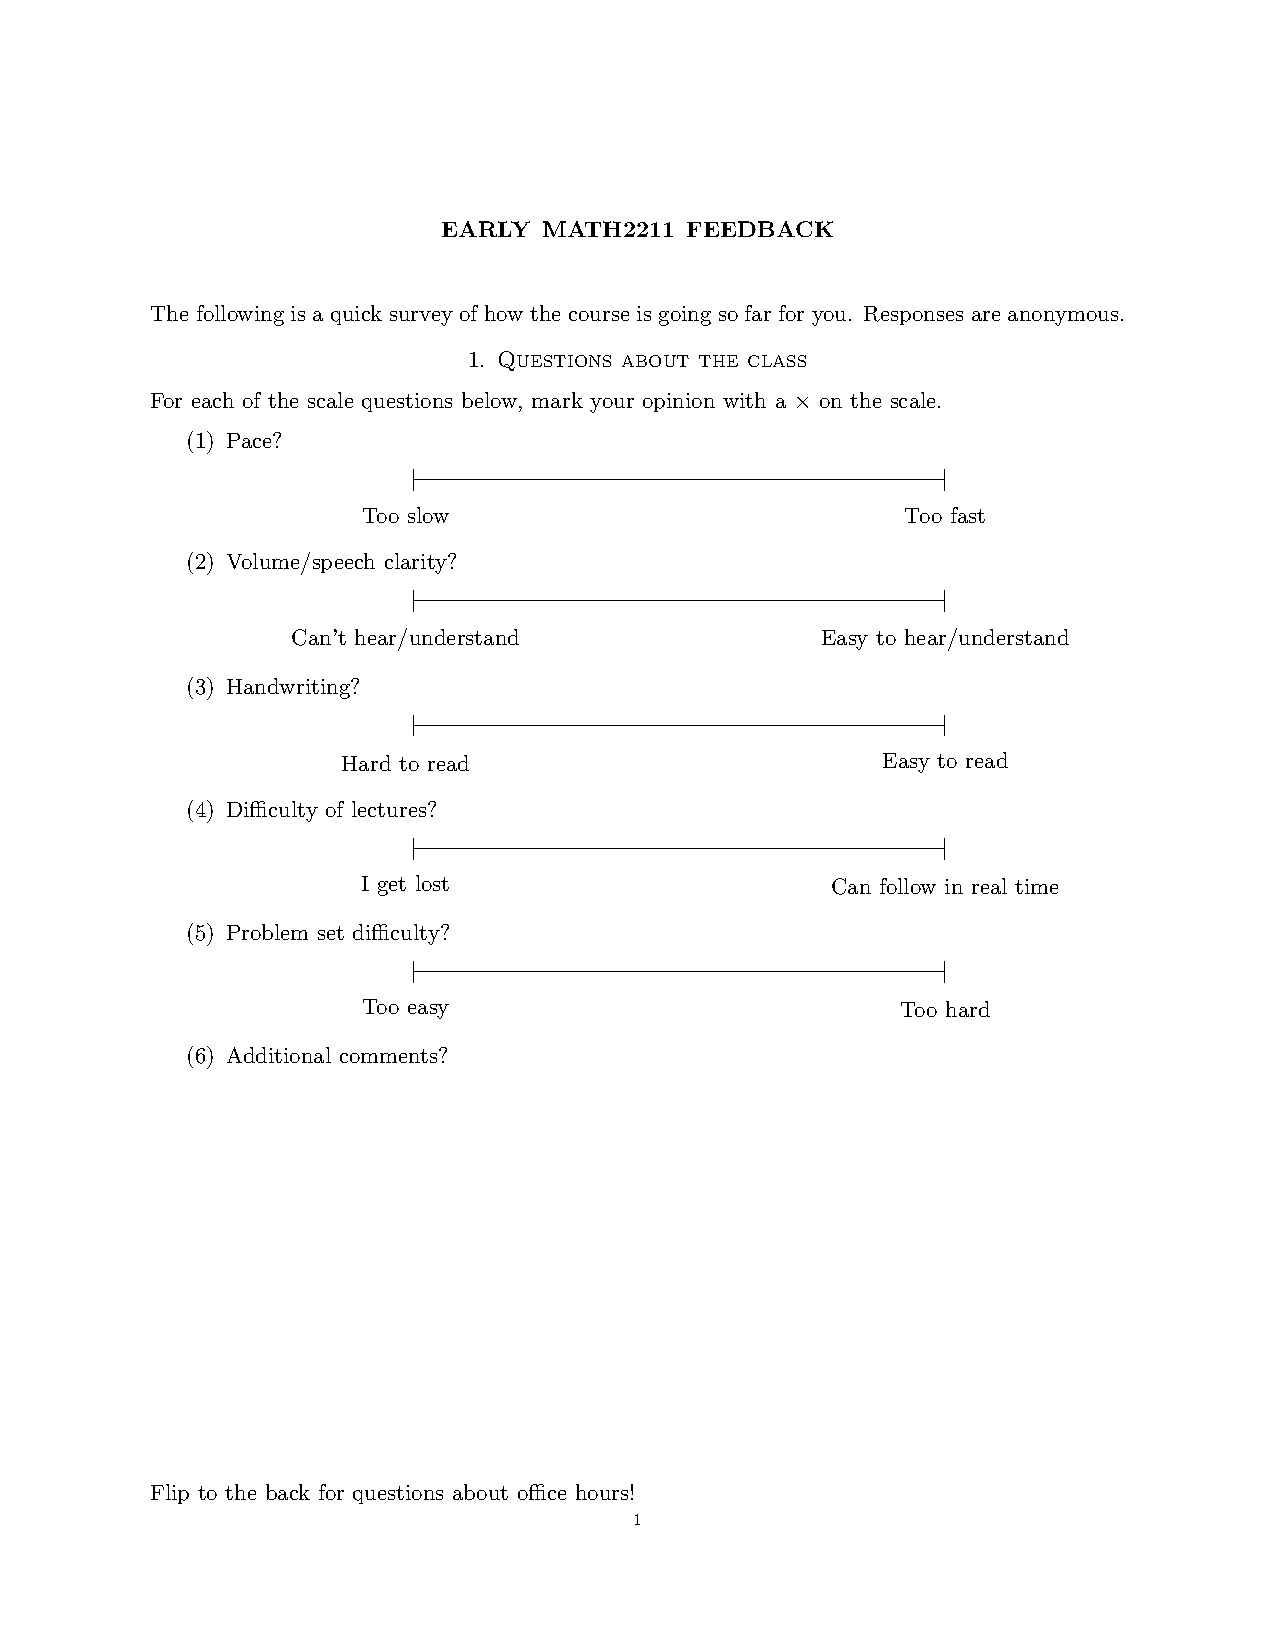
\includepdf[pages=-]{survey1.pdf}
\end{document}
